\documentclass{article}
\usepackage[utf8]{inputenc}

\title{A Keyword-Based UDP Hole Punching System for File Transfers}
\author{Austin Spadaro \\ Daniel Selmon \\ Wayne Chang}
\date{May 5th, 2013}

\usepackage{natbib}
\usepackage{graphicx}

\begin{document}

\maketitle

\section{Motivation}
Peer-to-peer communication is becoming increasingly popular with the explosion of networked devices. It not only saves expensive server bandwidth, but also has potential to provide lower latency and higher availability to all clients. These benefits are highly evident in popular p2p protocols such as BitTorrent and gnutella. However, there is a major drawback--the implementation of peer-to-peer systems is typically very difficult due to many network and security factors. The issue this paper attempts to overcome is called Network Address Translation (NAT).

\subsection{Network Address Translation}
Network Address Translation is a process that routers routinely use to modify header information within IP packets. This is a popular technique to provide network access to many nodes when only given one interface (for example, computers in a home to a single internet connection). Many nodes may "share" an out-facing interface. This process is problematic for p2p communications because the nodes behind the NAT may begin outgoing connections, but they cannot receive incoming connections in most configurations (this is possible in configurations such as port forwarding). Consequently, clients behind a NAT cannot accept incoming requests for data, but can only make requests to exchange resources. UDP hole-punching is one such solution to this problem.

\begin{figure}[h!]
\centering
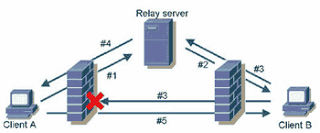
\includegraphics[scale=1]{UDP-Punching.png}
\caption{UDP Hole Punching}
\label{udphp}
\end{figure}

\section{UDP Hole Punching}
UDP hole-punching is a commonly employed NAT-traversal technique that allows incoming traffic to a client behind a NAT.

\subsection{UDP and NAT}
UDP packets are stateless and therefore do not have any sessions, but routers still must accommodate for two-way packet transfers over a NAT. Most routers do not allow incoming UDP packets initially, but do record the outgoing ports of UDP packets and the corresponding nodes on the LAN. This allows the router to anticipate a reply on those ports and correctly route the clients who have sent the requests. Fortunately, the destination addresses are not usually checked or recorded. This leniency is the basis for UDP hole punching.

\subsection{Steps}
UDP hole punching can be performed with two clients behind NATs/firewalls and a rendezvous server that can freely accept connections. First, the clients connect to the server and maintain the outgoing NAT ports with keep-alive packets. Then, the server knows each of the clients' NAT-translated addresses and source ports. Finally, the server exchanges the address and port information between the clients, allowing the clients to directly send packets to one another.

\subsection{Drawbacks}
Unfortunately, UDP hole punching does not work in all cases. In particular, it fails if the outgoing ports are randomized on a per-outbound host basis. It will also fail if the router or firewall employs tight security, requiring UDP source ports to only receive from addresses it has sent to. Despite its shortcomings, UDP hole punching is successful enough to be employed by popular services such as Skype and Hamachi.

\section{Implementation}

\subsection{Keywords}
This implementation uses a keyword-based system with clients in two possible modes. Keywords are used to denote a partial or full connection pair, and a connection pair consists of two clients: one in listen-mode and one in transfer-mode. The server maintains a list of active keywords. Clients in listen-mode may add a unique keyword to server, associating the keyword to its own address and source port. Clients in transfer-mode may send a request containing an existing keyword to the server and receive the associated address and port information. The keywords are secrets used by the clients in transfer-mode to unlock a destination address.

\subsection{Session Tracking}
The implementation allows for updated state information of connections in the server. Additional metadata is stored with the keyword to track connection state and time since last checkin. The connection states are heavily borrowed from TCP and will be described below in Messages. They allow for the server to track what the clients are currently doing. This information is convenient to display a list of active transfers or clients in listen-mode. In the implementation, the clients are trusted to deliver periodic status updates to the server containing their keywords. This allows for address updating.

\subsection{Address Updating}
Because UDP ports or addresses may change, it is important to keep track of the most current information per keyword. The status updates described above allows the server to update the keyword metadata for changed IP addresses or ports. If a client is running on a laptop or mobile devices moving through many networks, it can still reliably tell the server what its new address is. Clients in transfer-mode that stop receiving acknowledgement for data packets may request the server with the same keyword to see if there was change in address. 

\clearpage

\subsection{States}
Many of the states are mixed with messages. This should be changed in future revisions.
\begin{verbatim}
#define STATE_SYN       0
#define STATE_ACK       1
#define STATE_LISTEN    2
#define STATE_TRANSFER  3
#define STATE_FIN       4
#define STATE_SEND      5
#define STATE_ERROR     6
#define STATE_KEEPALIVE 7
\end{verbatim}

\subsection{Messages}
\begin{description}
\item[\textbf{SYN}] Clients in listen-mode send this message to initiate a keyword. Clients then receive an \texttt{ACK} containing the echoed keyword.  \\
\texttt{|------------------------------------------| } \\
\texttt{| 0 | null-terminated ascii keyword string | } \\
\texttt{|------------------------------------------| } \\
\item[\textbf{ACK}] An acknowledgement to \texttt{SYN} or keep-alives.
This confirms the keyword sent by SYN or keep-alives. \\
\texttt{|----------| } \\
\texttt{| 1 | data | } \\
\texttt{|----------| } \\
\item[\textbf{SEND}] Clients in transfer-mode send this message to receive a 7-byte response of \texttt{ACK}, IPv4 addres (4 bytes) and port (2 bytes) in network byte order. \\
\texttt{|------------------------------------------| } \\
\texttt{| 5 | null-terminated ascii keyword string | } \\
\texttt{|------------------------------------------| } \\
\item[\textbf{KEEPALIVE}] Clients in listen-mode or transfer-mode send this message to update state. \\
\texttt{|------------------------------------------| } \\
\texttt{| 5 | null-terminated ascii keyword string | } \\
\texttt{|------------------------------------------| } \\
\end{description}

\clearpage
\subsection{User Interface}
An example use of the system (in order):
\begin{description}
\item[\textbf{On the Server}] . \\
\texttt{./fpunchd 6699}

\item[\textbf{On the Client 1}] . \\
\texttt{./fpunchd listen mathbook}

\item[\textbf{On the Client 2}] . \\
\texttt{./fpunchd transfer mathbook linear_algebra.pdf}

\section{Future Work}
\subsection{Better Data Transfer}
Right now, the system only supports the sending of simple messages. The file transfer aspect was already covered in previous projects (TFTPD), but there is potential for much more. If a stream session was implemented over UDP with hole punching and a relay fall-back to the server, it could be very useful as a library in the implementaion of any p2p program. Such solutions already exist, and a project could be attempted for learning purposes or to discover novel techniques.

\bibliographystyle{plain}
\bibliography{references}
\end{document}

